\chapter{Experiments}

\section{Experiments with SSD}
\label{chapt:improvemnets}

\subsection{Building SSD on Resnet}
resnet
bla bla 10,18,32,50,101...

feature map sized
block1: 56x56
block2: 28x28
block3: 14x14
block4: 7x7

unlike original SSD on VGG-16 we decided to start with this basic setup without adding more feature layers, because we are interested in small objects on surveillance video and not for recognizing large objects on photographs.

\begin{figure}
    \centering
    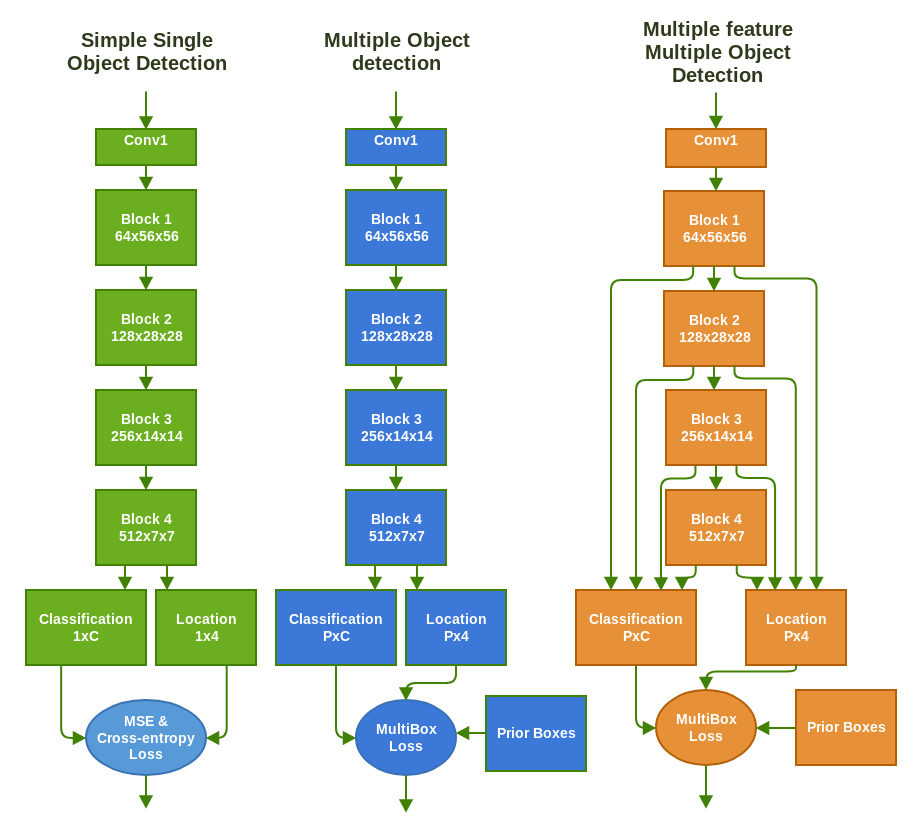
\includegraphics[width=\textwidth]{img/resnets.png}
    \caption{High level structure of resnet with SSD}
    \label{fig:resnet}
\end{figure}




\subsubsection{artificial dataset}
random generated circles, triangles and squares with random size and color, triangles are randomly rotated. placing random object over a background of random lines generated by using the same types of objects but upscaled so they are not fully in the image. Object for detection is drawn on top. 

\subsubsection{Simple detector for one object}

optimizer = Adam(lr=0.001, betas=(0.9, 0.999), eps=1e-08, weight decay=0)
class loss = CrossEntropyLoss
loc loss = MSELoss output of NN with absolute coordinates of ground truth box normalized to -1,1 

resnet 18: in addition to fully connected layer we use feature map before avg pooling as input to 7x7 convolution with 4 filters (4 coordinates) Only output of B4 on picture \cref{fig:resnet} 

test on 10000 images
results: class accuracy: over 99.73\%
class loss: 0.0132
location loss (mean squared error): 0.0043


\begin{figure}
    \centering
    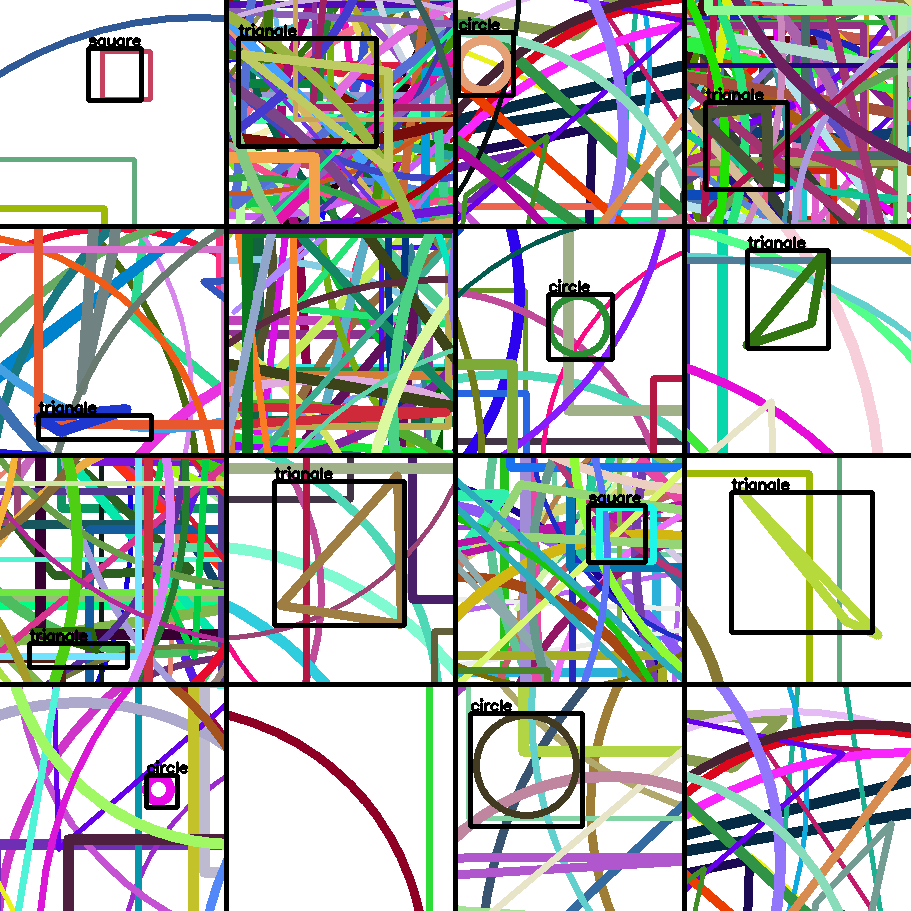
\includegraphics[width=\textwidth]{img/simple_detection.png}
    \caption{Detections by simple model 1 7x7 feature map to 4 coordinates and fully connected for class}
    \label{fig:my_label}
\end{figure}

\subsubsection{Adding priorboxes}

\subsubsection{Full SSD, convolution and multiple feature layers}


\subsection{Applying SSD trained on artificial dataset to realistic images}

\subsection{Measuring the impact of number of classes}

\section{Speeding up video procesing}